\documentclass{beamer}

\input defs.tex
\input formatting.tex
\newcommand{\citet}[1]{{\footnotesize{\textmd{[#1]}}}}

%\mode<handout>
\mode<presentation>
{
\usetheme{default}
}
\setbeamertemplate{footline}[frame number]

\usepackage{amsmath,amsthm,comment,mathtools}
\usepackage{array,graphicx,amssymb,psfrag}
\usepackage{caption,subcaption}
\usepackage{algorithm,algorithmicx,algpseudocode}
\usepackage{epstopdf}
\epstopdfsetup{update}
\usepackage{tikz}
\usetikzlibrary{shapes}
\usepackage{pgfplots}
\pgfplotsset{compat=newest}
\pgfplotsset{every axis legend/.append style={%
cells={anchor=west}}
}
\usetikzlibrary{arrows}
\tikzset{>=stealth'}
\pgfplotsset{width=12cm}

\bibliographystyle{alpha}

\title{ORIE 4741: Introduction to AutoML}

\date{\textcolor{blue}{October 28, 2019}}
\author{Chengrun Yang \\
	[1ex]
%	Operations Research and Information Engineering \\
}

\begin{document}

\begin{frame}
%
\includegraphics[width=.12\linewidth]{cornell_seal.pdf}
\titlepage
\end{frame}


 \begin{frame}{Outline}
 \tableofcontents
 \end{frame}

\section{Motivation}

\begin{frame}{What would we do to select models?}
Model: algorithm + hyperparameter settings

e.g. ridge regression with $\lambda = 1$
\vfill
In supervised learning, given a training set $ \{(x_i, y_i)\} $ and test points $ \{x_j\} $, how would we get $ \{y_j\} $?
\pause
\bit
\item linear regression?
\item random forest?
\item gradient boosting?
\item \dots
\item try all the models in scikit-learn \cite{scikit-learn}, or all the available neural network architectures?

\eit
\end{frame}

\begin{frame}{Model selection is important}
A naive exhaustive search that runs all models wastes
\bit
\item programmer time
\item computational time
\bit
\item[$\cdot$] takes long on small datasets
\item[$\cdot$] is impossible on large datasets
\eit
\eit

\vfill
Approaches to avoid exhaustive search:
\bit
\item single dataset: surrogate models to predict performance
\bit
\item Gaussian processes
\item genetic programming
\eit
\item learn across datasets: meta-learning
\eit

%AutoML: a relatively young field
\end{frame}

\begin{frame}{Learning vs meta-learning}
\begin{figure}
	\begin{subfigure}[t]{0.48\linewidth}
		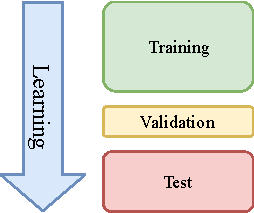
\includegraphics[width=0.8\linewidth]{learning.pdf}
		\caption{Learning}
	\end{subfigure}
	\begin{subfigure}[t]{0.48\linewidth}
		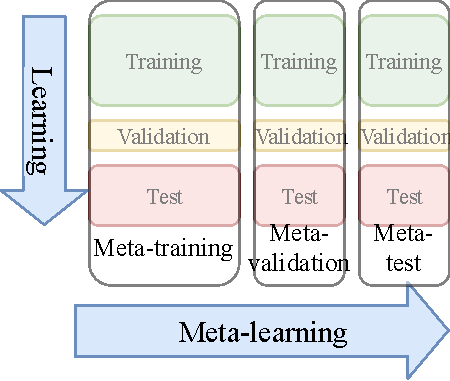
\includegraphics[width=0.8\linewidth]{meta_learning.pdf}
		\caption{Meta-learning}
	\end{subfigure}
\end{figure}
\end{frame}



\section{Some AutoML systems}
\begin{frame}{AutoML frameworks for general models}
\bit
\item Bayesian optimization frameworks \cite{snoek2012practical, klein17a, zhang2016flash, thornton2013auto} \dots
\item auto-sklearn \cite{feurer2015efficient}: meta-learning + Bayesian optimization
\item TPOT \cite{Olson2016EvoBio}: genetic programming
\item H2O AutoML
\item Hyperband \cite{JMLR:v18:16-558}
\item Probabilistic matrix factorization (PMF) \cite{fusi2018probabilistic}
\item \textsc{Oboe}: matrix factorization + experiment design \cite{yang2019oboe}
\item $\cdots$
\eit

\end{frame}

\begin{frame}{AutoML for neural architecture search}
Techniques in use:
\bit
\item reinforcement learning \cite{45826} \dots
\item genetic programming \cite{suganuma2017genetic} \dots
\item Bayesian optimization \cite{Jin:2019:AEN:3292500.3330648} \dots
\item $\cdots$
\eit
\end{frame}



\section{Demo!}
\begin{frame}{Question: When does AutoML overfit?}
Recall overfitting: low training error and high test error
\end{frame}

\begin{frame}[allowframebreaks]{References}
\bibliographystyle{alpha}
\bibliography{scholar}
\end{frame}

\end{document}
